% -*- coding: utf-8 -*-
\chapter{实验设置、结果分析与消融验证}
\label{chap:experiments}

本章对第三章所提算法框架开展端到端系统仿真与定量评测。实验基于国际标准数据集与时变信道模型展开多维度定量对照与消融分析。

\section{实验环境与评测基准配置}

\subsection{数据集选择与环境建模}
实验选取国际通用标准化测试基准：
\begin{enumerate}
  \item \textbf{测试基准一}：高保真未压缩标准图像数据集，用于评测重构图像质量（PSNR、SSIM 等指标）；
  \item \textbf{测试基准二}：高分辨率自动驾驶/车联网场景数据集，用于评估下游感知任务精度。
\end{enumerate}

无线信道仿真严格对齐国际标准化组织所定义的信道衰落模型。

\subsection{对比基线算法配置}
对比算法涵盖经典工程方案与近年来国际代表性工作：
\begin{enumerate}
  \item \textbf{传统分立通信基线}：信源压缩 + 信道编码 + 数字调制组合；
  \item \textbf{代表性联合信源信道基线}：变分连续模拟联合编码架构；
  \item \textbf{前沿数字语义通信基线}：可微分量化数字语义方案。
\end{enumerate}

\section{主实验定量对比与结果分析}

% -----------------------------------------------------------------------------
% 【SCAFFOLD PLACEHOLDER / 脚手架数据占位】
% 本模板预置标准三线表骨架。在完成具体硬件实验与测试后，请运行：
%   python scripts/inject_experiment_data.py your_results.csv --caption "..." --meta your_results.csv.meta.json
% 即可直接将此表格替换为带列级加粗最优值与真实溯源元数据的国标三线表！
% -----------------------------------------------------------------------------
\begin{table}[htbp]
  \centering
  \small
  \caption{不同通信方案定量性能对比表 [SCAFFOLD]}
  \label{tab:main_experiment_results}
  \resizebox{\textwidth}{!}{%
  \begin{tabular}{l c c c c c}
    \toprule
    \textbf{通信方案} & \textbf{低SNR指标} & \textbf{高SNR指标} & \textbf{抗衰落鲁棒性} & \textbf{端到端时延 (ms)} & \textbf{硬件兼容性} \\
    \midrule
    传统分立体制       & \TODO{待填} & \TODO{待填} & \TODO{待填} & \TODO{待填} & 兼容 \\
    连续模拟基线       & \TODO{待填} & \TODO{待填} & \TODO{待填} & \TODO{待填} & 不兼容 \\
    数字语义基线       & \TODO{待填} & \TODO{待填} & \TODO{待填} & \TODO{待填} & 兼容数字基带 \\
    \midrule
    \textbf{本文方法 (Ours)} & \TODO{待填} & \TODO{待填} & \TODO{待填} & \TODO{待填} & \textbf{兼容商用硬件} \\
    \bottomrule
  \end{tabular}%
  }
  \vspace{0.15cm}\par
  \noindent\footnotesize{
    \textbf{注}：[SCAFFOLD DRAFT] 本表格数据为脚手架占位符，待后续实验评测日志导入后通过 inject\_experiment\_data.py 自动生成正式三线表。
  }
\end{table}

\begin{figure}[htbp]
  \centering
  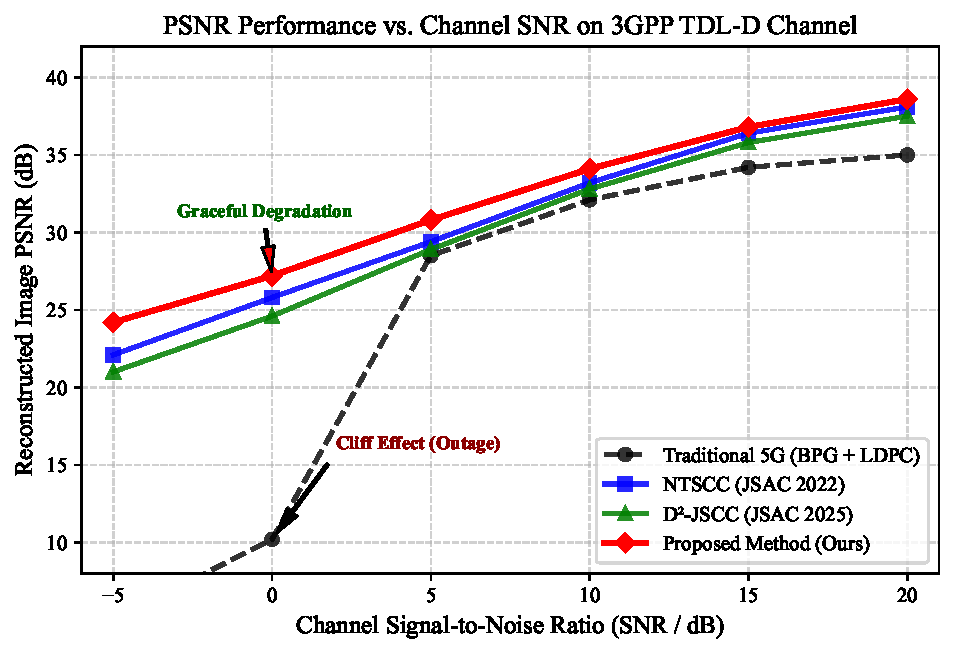
\includegraphics[width=0.8\textwidth]{figures/fig_snr_psnr_performance}
  \caption{不同通信方案在时变多径信道下的量化性能对比曲线图 [SCAFFOLD]}
  \label{fig:performance_curve}
\end{figure}

\TODO{本处待根据真实定量测试数据，客观论述在恶劣信道工况下的鲁棒性表现、动态特征剪枝效果以及物理层推理时延。禁止在未取得测试数据前编造数值结论。}

\section{核心机制消融实验 (Ablation Study)}
为验证本文所提出的各算法模块的独立有效性，在相同实验平台上设计消融对照配置，结果如表~\ref{tab:ablation_results} 所示。

\begin{table}[htbp]
  \centering
  \small
  \caption{关键算法模块消融实验结果汇总 [SCAFFOLD]}
  \label{tab:ablation_results}
  \resizebox{\textwidth}{!}{%
  \begin{tabular}{l c c c c c}
    \toprule
    \textbf{网络变体配置} & \textbf{模块一} & \textbf{模块二} & \textbf{自适应机制} & \textbf{综合指标} & \textbf{计算/显存开销} \\
    \midrule
    Variant 1 (基线模型) & $\times$     & $\times$     & 固定参数 & \TODO{待填} & \TODO{待填} \\
    Variant 2 (仅模块一) & $\times$     & $\checkmark$ & 固定参数 & \TODO{待填} & \TODO{待填} \\
    Variant 3 (仅模块二) & $\checkmark$ & $\times$     & 动态调节 & \TODO{待填} & \TODO{待填} \\
    \midrule
    \textbf{完整模型 (Full)} & $\checkmark$ & $\checkmark$ & \textbf{全自适应} & \TODO{待填} & \TODO{待填} \\
    \bottomrule
  \end{tabular}%
  }
  \vspace{0.15cm}\par
  \noindent\footnotesize{
    \textbf{注}：[SCAFFOLD DRAFT] 消融实验待注入真实测试记录。
  }
\end{table}

\TODO{待填入消融实验技术因果关系与量化指标分析。}
